Dta miners find generalizations (a.k.a. summaries)
of the data. All such generalizations must be smaller than the data it generalizes (otherwise we might as well just keep the original data and ignore the generalization)\footnote{Technical note:
even instance-based reasoners uses generalizations when they partially match new cases to old;
or if they use some  clustering algorithm to restrict the case matching
to just the subset of old cases most similar  to new  cases.}. 
Generalization is important since,
without generalization, all we can do is perform exact matches
of new situations to a database of old examples. This is not recommended practice since,
 if the new situation has not occurred  before, then nothing in the data  will
 matches the new situation
(and we cannot make any predictions).

The key point here is that there are many ways to summarize data and exceConsider some learner that
builds predictive rules form a subset of  attributes $A$ ranges. Assuming numeric attributes
divided into five ranges, then the 20 attributes of \fig{ck} can be combined into 
$2^{5*20}> 10^{30}$
possible rules 

\section{Algorithm: Predictor and Tuner}

In order to conduct the experiment of this paper, we need one tool that can predict defects 
from the empirical data sets and a second tool to tune the built-in parameters associated with 
predictor. To compare the effects of the tuning process, we have three different predictors: 
WHERE-based Predictor, CART and Random Forest. Different Evolution(DE) as an optimizer 
is used as a tuner in this paper.

We choose CART and Random Forest as a predictor in this paper is motivated by 
\cite{lessmann2008benchmarking}, where the performance of both tools as predictors are 
significantly different based on authors' experiment as mentioned before. We'd like to 
investigate whether tuning can change such conclusion. WHERE-based Predictor is a new 
defect predictor based on WHERE\cite{menzies2013local} algorithm. A comparison with 
standard predictor like CART and Random Forest will better evaluate and judge the 
performance such new predictor. As for the tuner, there're many heuristic optimization 
algorithms in wild. However, DE is a good but maybe not the best candidate for the tuning 
process considering different performance measurements. To determine which optimizer is 
fitable and results in better performance is beyond this work scope. We leave it to future 
works. The rest of this section will describe each tool applied in this work.

 \subsection{WHERE-based Learner}
\textbf{WHERE-based Learner} is composed of WHERE clustering algorithm and CART 
decision tree algorithm. The key idea of WHERE-based learner is that  instead of training the 
CART decision tree based on the class labels associated with each training sample, it's using 
CART to build decision trees based on the cluster labels, which are generated by the WHERE 
clustering algorithm.
 
 
 
\begin{figure}[!t]

\renewcommand{\baselinestretch}{0.8}
\scriptsize
\centering
  \begin{tabular}{r@{~}|r@{~}rr|r@{~}rr|r@{~}rr}
    & \multicolumn{3}{c|}{WHERE}&\multicolumn{3}{c|}{CART}& \multicolumn{3}{c}{Random Forest}\\\cline{2-10} 
    Goal & tuned & naive &$\frac{\mathit{tuned}}{\mathit{naive}}$& tuned & naive &$\frac{\mathit{tuned}}{\mathit{naive}}$& tuned & naive&$\frac{\mathit{tuned}}{\mathit{naive}}$\\\hline
pd&71.4&1.2&60&4.4&0.1&44&7.1&0.2&36\\ 
prec&82.8&1.4&59&3.9&0.1&39&7.4&0.2&37\\
f&86.1&1.2&72&3.3&0.1&33&6.7&0.2&34
  \end{tabular}
  \caption{For one train/test set pair (ANT),  time (in seconds) spent tuning,
  for different goals, or just running the ``off-the-shelf'' learner.}
\end{figure}


\begin{figure}[!t]

\renewcommand{\baselinestretch}{0.8}
\scriptsize
\centering
\begin{tabular}{r|rrr}
goal &	WHERE	&CART&	Random Forest\\\hline
f	&15	&13	&9\\ 
pd	&15	&16	&8\\ 
prec&	14	&14	&8
\end{tabular}
\caption{How much slower is tuning vs just running the default
settings of the learner? E.g. bottom right, tuning to increase
precision with Random Forests is eight times slower than
just running Random Forests.}
\end{figure}



% Given N instances, instead of building decision tree directly with CART, we use WHERE to 
%cluster instances. 
WHERE is a fast clustering algorithm designed by {\it menzies} for finding software artifacts 
with similar attributes. It clusters data on dimensions synthesized along the axis of greatest 
variability in the data. The way WHERE used to find such dimension is a linear-time heuristic 
called ``FASTMAP" proposed by Faloutsos \& Lin\cite{faloutsos1995fastmap}. ``FASTMAP" 
randomly picks one instance $Z$; find the instance {\it east} $X$ that's furthest away form $Z$; find 
the instance {\it west} $Y$ that's furthest away from {\it east} $X$. Next, project all the remaining 
points onto the line drawn between $X$ and $Y$.  The line $\overline{XY}$ is an approximation of the 
first component found by PCA. As shown in Figure \ref{Where}, $X$ and $Y$ are the furthest points found by ``FASTMAP'' and $\overline{XY}$ is of length $c$. Each point in this figure has a distance $a$
to $X$ and distance $b$ to $Y$. According to the coisne rule and Pythagoras, each instance will be mapped 
into 2-dimension by the following equations.
\begin{equation}
\begin{split}
x  &= (a^2 +c^2-b^2)/(2c)\\ 
   y  &= \sqrt{a^2 -x^2}
\end{split}
\end{equation}


Then choose the median point $\hat{x}$ as the split and 
recursively divide all the instances into {\it west} and {\it east} clusters until the number of 
instances within each cluster is less than specific minimum size. The representation of the 
clustering result is a tree, we call it Where-clustering tree. Such tree will be pruned if applicable 
in some cases. Finally, cluster labels  will be assigned to instances in each of those 
clusters(leaves). 

\begin{figure}[!ht]
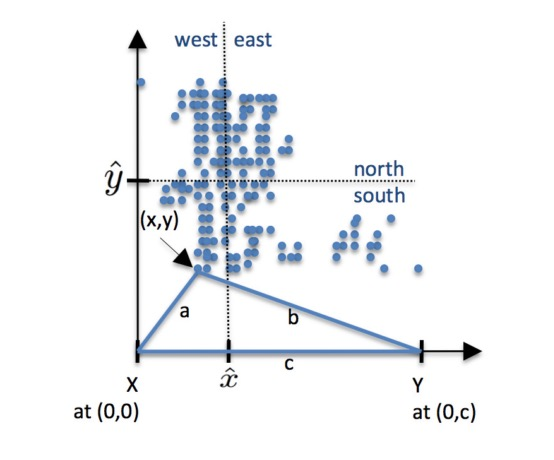
\includegraphics[scale=0.5]{where.png}
\caption{WHERE algoirthm }
\label{Where}
\end{figure}
Then based on the attributes and the cluster labels in each instances,  we build a 
decision tree based on CART algorithm. In each leaf of the tree, there're several instances 
falling in. This will be the model trained for defect prediction. During testing process, a new 
instance comes in and traverses the tree according to 
values of the its attributes. If the instance could reach one leaf of the tree, the predicted value 
of this instance will be the mean  of all the training data values associated with this leaf. 
Otherwise if stops at intermediate nodes of tree, the predicted value will be the mean of the all 
the training data value below this node. After estimating all the number of defectives in the test 
data, whether each instance contains defectives will be determined by comparing with a threshold value. If the predicted value is greater than threshold, the Where-based learner will predict this instance as defective otherwise non-defective.


%\begin{algorithm}
%	\caption{Pesudocode for WHERE Algorithm }
%	\label{alg:WHERE}
%	\begin{algorithmic}[1]
%	\Require $data$
%	\Ensure $tree$
%	\Function {Fastmap}{$ data$}
%	\State $one \gets$ any$(data)$
%	\State $west \gets$ furthest$(data, one)$
%	\State $east \gets$ furthest$(data, west)$
%	\State $c \gets$ distance($west, east$)
%	\EndFunction
%	\end{algorithmic}            
%\end{algorithm}

\subsection{CART}
\textbf{CART} is an {\em iterative dichotomization} algorithm
that finds the attribute that most divides the data such that
the variance of the goal variable in each division is
minimized\cite{breiman84}.
The algorithm then recurses on each division.
Finally, the cost data in the leaf divisions
is averaged to generate the estimate.

\subsection{Random Forests}

Breiman's website describes \textbf{Random Forests} as
follows\cite{brieman00}. "Random Forests grows many classification
trees. To classify a new object from an input vector, put the input
vector down each of the trees in the forest. Each tree gives a
classification, and we say the tree "votes" for that class. The forest
chooses the classification having the most votes (over all the trees
in the forest). Each tree is grown as follows.
If the number of cases in the training set is N, sample N cases at
random - but with replacement, from the original data. This sample
will be the training set for growing the tree.
Also, if there are M input variables, a number m$<<$M is specified such
that at each node, m variables are selected at random out of the M and
the best split on these m is used to split the node. The value of m is
held constant during the forest growing.
Finally, each tree is grown to the largest extent possible (there is
no pruning)."




%Suppose the cordinates of X and Y are $(0,0)$ and $(0,c)$, which are east and west 
%instances within N samples. From the Pythegoras and cosine rule, each instance is projected 
%at the point(x,y)
%
%\begin{equation}
%	\begin{split}
%	x &= (a^2 + c^2 - b^2)/(2c) \\
%	y &= \sqrt{a^2 - x^2} 
%	\end{split}
%\end{equation}

